\section{Results}
\label{sec:results}

We report mean and standard deviation over 8 seeds. Table~\ref{tab:main} gives
the continual-learning metrics, Table~\ref{tab:baselines} the non-learning
baselines, and Table~\ref{tab:sig} the paired significance tests. We present the
results as measured, including where they do not confirm our expectations.

\subsection{Learning within a phase}
Figure~\ref{fig:learning} shows the greedy evaluation reward on phase~0 as a
function of training episodes. The agent starts near the random level and rises
toward the \textsc{greedy-create} reference, confirming that the RL loop solves
the within-phase problem before we ask it to learn across phases.

\begin{figure}[t]\centering
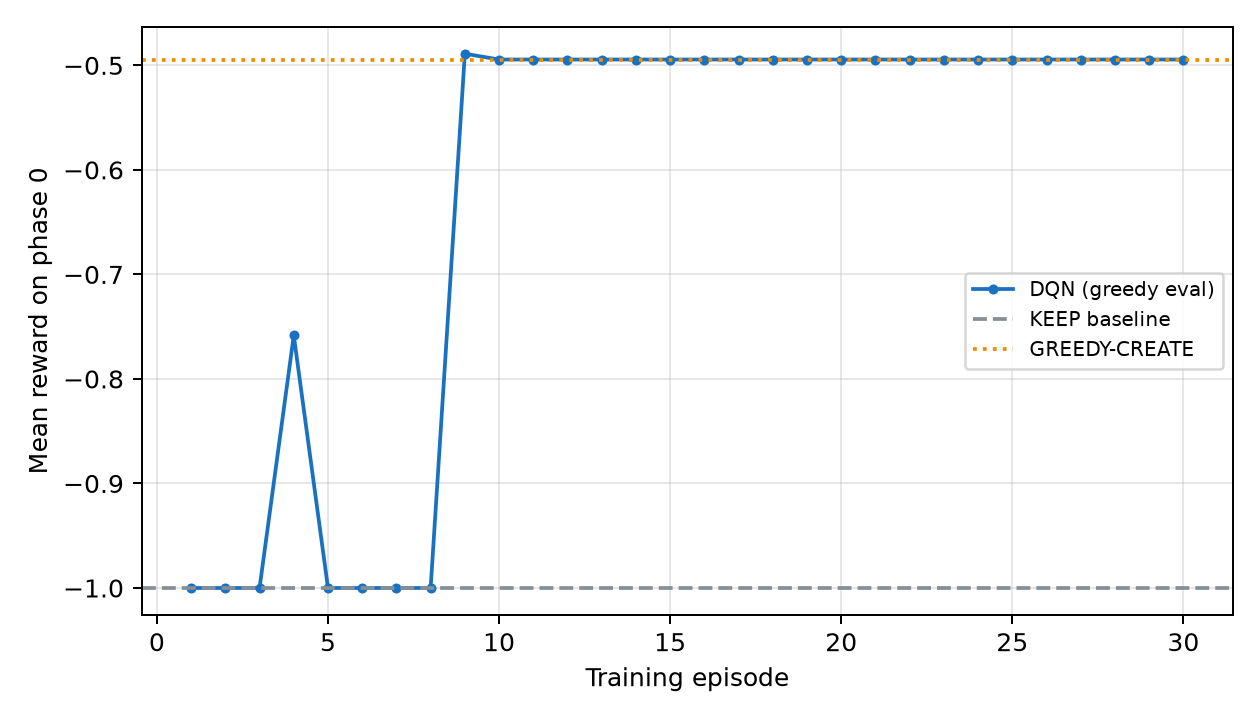
\includegraphics[width=\linewidth]{figures/fig_learning_curve.png}
\caption{Single-phase learning curve (DQN on phase 0) against static baselines.}
\label{fig:learning}
\end{figure}

\subsection{Baselines}
\begin{table}[t]\centering\small
\caption{Baseline per-phase reward (mean over seeds). Higher is better.}
\label{tab:baselines}
\begin{tabular}{lrrrrrrrr}
\toprule
Method & T0 & T1 & T2 & T3 & T4 & T5 & T6 & Mean \\
\midrule
KEEP & -1.00 & -1.00 & -1.00 & -1.00 & -1.00 & -1.00 & -1.00 & -1.00 \\
RANDOM & -0.86 & -0.88 & -1.34 & -0.89 & -1.33 & -1.32 & -0.87 & -1.07 \\
GREEDY-CREATE & -0.50 & -0.50 & -1.40 & -0.50 & -1.40 & -1.40 & -0.50 & -0.88 \\
\bottomrule\end{tabular}\end{table}

KEEP (never index) is uniformly poor: every query pays the high latency
(\(\approx-1.0\)). RANDOM is dragged down by the conflict phases, where indexing
is actively harmful (\(\approx-1.3\)). GREEDY-CREATE indexes whenever structurally
possible; it is optimal on the selective phases but is the \emph{worst} method on
the conflict phases, because it confidently builds indexes that cannot help. This
is the central practical hazard: a policy tuned to yesterday's workload can be
worse than doing nothing after the workload drifts, which is precisely why an
adaptive, forgetting-aware agent is needed.

\subsection{Continual-learning metrics}
\begin{table}[t]\centering\small
\caption{Continual-learning metrics (mean $\pm$ std over 8 seeds). ACC/BWT/FWT/F per Lopez-Paz \& Ranzato.}
\label{tab:main}
\begin{tabular}{lrrrr}
\toprule
Method & ACC & BWT & FWT & Forgetting $\mathcal{F}$ \\
\midrule
CLDB-RL (EWC+Prioritized) & $-0.954\pm0.041$ & $-0.076\pm0.067$ & $0.189\pm0.035$ & $0.125\pm0.062$ \\
RL (no EWC) & $-0.919\pm0.058$ & $-0.035\pm0.080$ & $0.183\pm0.035$ & $0.105\pm0.081$ \\
RL (online, no replay) & $-1.000\pm0.000$ & $-0.197\pm0.031$ & $0.265\pm0.031$ & $0.198\pm0.031$ \\
\bottomrule\end{tabular}\end{table}

\paragraph{Replay prevents catastrophic forgetting.}
The replay-free online agent collapses: its final performance is the KEEP level
on every phase, \mbox{\(\mathrm{BWT}=-0.197\pm0.031\)} and
\mbox{\(\mathcal{F}=0.198\pm0.031\)}, with remarkably small variance across seeds.
Both replay-based agents reduce forgetting by roughly a factor of two
(\(\mathcal{F}=0.125\pm0.062\) and \(0.105\pm0.081\)) and improve the final
average reward (\(\mathrm{ACC}\)). The paired tests (Table~\ref{tab:sig}) confirm
that forgetting is significantly lower for a replay-based agent than for the
online agent (\(\text{CLDB-RL vs. online } p=0.037\);
\(\text{no-EWC vs. online } p=0.039\)). This is the paper's headline result and
it is robust: rehearsal is what stops the collapse.

\paragraph{EWC's incremental benefit is not established here.}
Contrary to our expectation, adding drift-triggered EWC does \emph{not}
significantly improve on replay alone in this benchmark (CLDB-RL vs.\ no-EWC,
\(p=0.319\)); its forgetting is nominally slightly higher. We attribute this to
over-regularization: with seven conflicting phases and a quadratic Fisher
penalty accumulated over many consolidations, the anchor can slow re-learning of
the current phase. This is a negative result we report explicitly; it does not
invalidate EWC in general (Proposition~\ref{prop:drift} shows the trade-off is
controlled by \(\lambda\), which we did not tune) but it means EWC should not be
claimed as the source of CLDB's robustness on this benchmark.

\paragraph{Learned vs.\ heuristic.}
On raw reward the learned agents (\(\mathrm{ACC}\approx-0.92\) to \(-0.95\)) do not
beat GREEDY-CREATE (\(\approx-0.88\)): both fail to suppress indexing on the
conflict phases, where the optimal action is KEEP. They comfortably beat KEEP and
RANDOM. Thus CLDB's advantage over the heuristic is \emph{not} in peak reward but
in the properties a heuristic lacks---it is learned from reward without
hand-coded rules and, critically, it can continue to adapt without the
catastrophic collapse exhibited by the online control.

\subsection{Retention and the \(R\)-matrix}
\begin{figure}[t]\centering
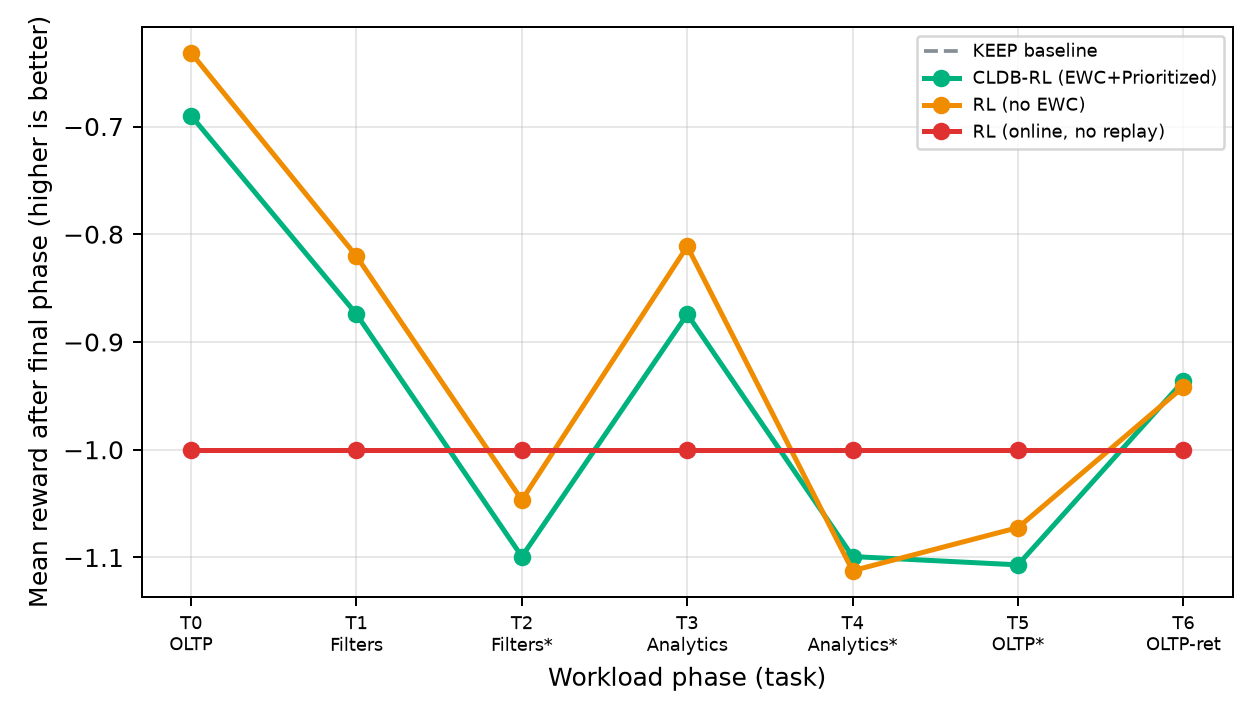
\includegraphics[width=\linewidth]{figures/fig_retention.png}
\caption{Final greedy reward per phase (higher is better).}
\label{fig:retention}
\end{figure}

\begin{figure*}[t]\centering
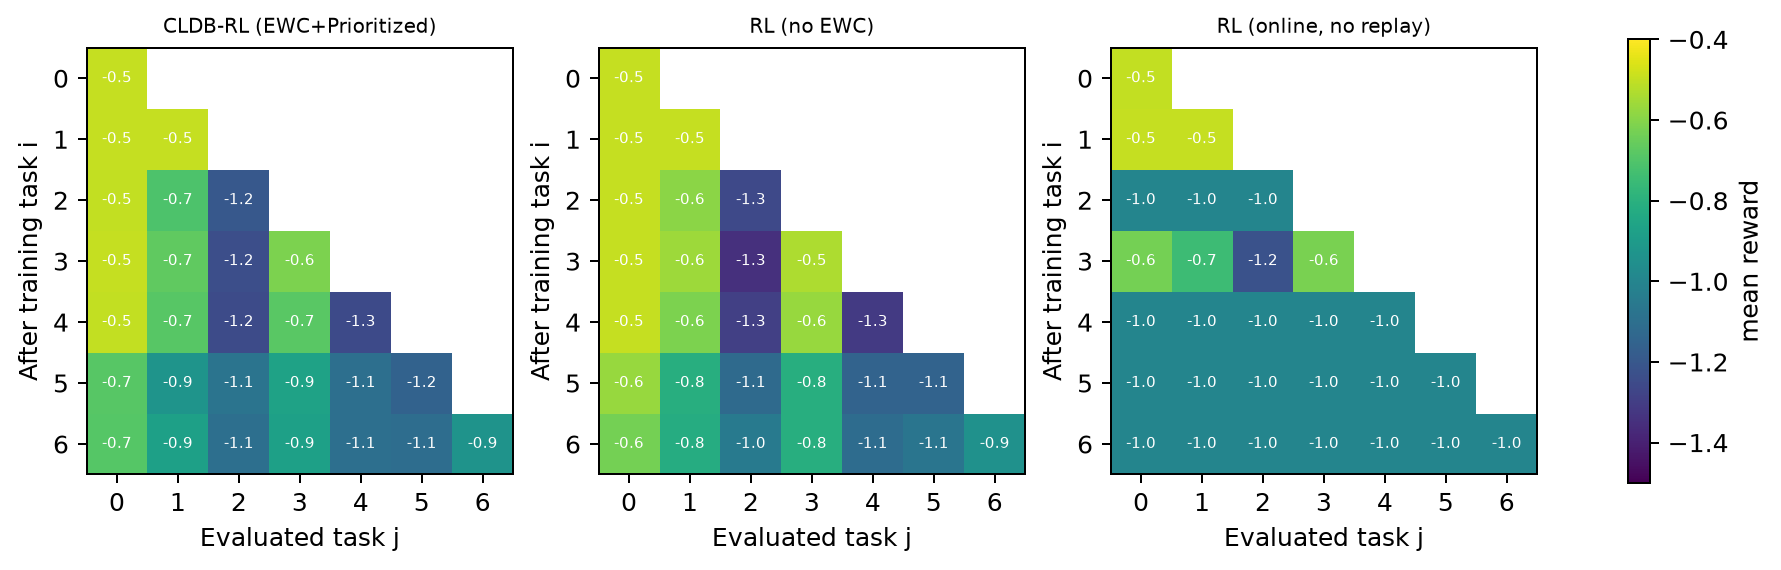
\includegraphics[width=\textwidth]{figures/fig_rmatrix.png}
\caption{Evaluation matrices $\R$ ($R_{i,j}$ = reward on phase $j$ after training
phase $i$). Bright cells indicate retained competence. The online agent (right)
loses previously learned phases; replay-based agents (left, centre) retain more.}
\label{fig:rmatrix}
\end{figure*}

Figure~\ref{fig:retention} shows final performance per phase; the replay-based
agents track the structure of the phase landscape (good on selective phases,
poor on conflict phases) whereas the online agent is flat at the KEEP level,
having forgotten how to index usefully. Figure~\ref{fig:rmatrix} shows the full
evaluation matrix \(\R\). The online agent exhibits the signature of catastrophic
forgetting: rows that were strong immediately after learning a phase decay to the
KEEP level as subsequent phases are learned. The replay-based matrices retain
bright structure for earlier phases.

\subsection{Summary}
The stable, reproducible findings are: (i) an online index agent forgets
catastrophically under workload drift; (ii) a replay buffer significantly reduces
forgetting; (iii) drift-triggered EWC gives no significant additional benefit at
the untuned \(\lambda\) we used; and (iv) the learned agent matches a structural
heuristic on reward while remaining adaptive and now no longer collapses. Effect
sizes are modest because the benchmark is deliberately small; the \emph{direction
and consistency} across seeds, supported by paired tests, is the claim.
